\documentclass[14pt,a4paper]{extarticle}
\usepackage[T2A]{fontenc}
\usepackage[utf8]{inputenc}
\usepackage[english,russian]{babel}
\usepackage{lmodern}
\usepackage{geometry}
\usepackage{array}
\usepackage{tabularx}
\usepackage{longtable}
\usepackage{ltablex}
\usepackage{booktabs}
\usepackage{hyperref}
\usepackage{indentfirst}
\usepackage{microtype}
\usepackage{graphicx}
\usepackage{setspace}
\usepackage{listings}
\usepackage{graphicx}
\usepackage{caption}
\usepackage{float}
\usepackage{tocloft}
\usepackage{titlesec}
\usepackage{newtxtext,newtxmath}

\titleformat{\section}        % форматируем \section
  {\normalfont\bfseries}      % стиль: обычный + жирный
  {\thesection.}              % номер секции с точкой
  {2mm}                       % расстояние между номером и текстом
  {}                           % перед заголовком можно добавить что-то
\titlespacing*{\section}{1.5cm}{*3}{*1}  % {отступ слева}{отступ сверху}{отступ снизу}

\captionsetup{justification=centering}
\renewcommand{\ttdefault}{cmtt}
\keepXColumns
\setlength{\parindent}{3em}
\newgeometry{left=2.5cm,right=2.5cm,top=3cm,bottom=2.5cm}

\renewcommand{\contentsname}{\hspace*{4em}{\smallСодержание}}
\setlength{\cftbeforesecskip}{0.5em}
\renewcommand{\cftsecleader}{\cftdotfill{\cftdotsep}}
\renewcommand{\cftsecaftersnum}{.\hspace{2mm}}

\title{Отчёт по дисциплине "Системная инженерия"}
\author{Выполнил студент группы М-РИТ-25-1, Станиславчук Сергей}

\begin{document}

\setstretch{1.5}
\noindent
\begin{minipage}[t]{0.01\textwidth}
    \includegraphics{~/programmer/++Programmer/5_1/LSTU.jpg}
\end{minipage}%
\begin{minipage}[c]{1.1\linewidth}
    \centering
    {\small
    МИНИСТЕРСТВО НАУКИ И ВЫСШЕГО ОБРАЗОВАНИЯ РФ \\[1em]
    ФЕДЕРАЛЬНОЕ ГОСУДАРСТВЕННОЕ БЮДЖЕТНОЕ \\
    ОБРАЗОВАТЕЛЬНОЕ УЧРЕЖДЕНИЕ ВЫСШЕГО ОБРАЗОВАНИЯ \\
    «ЛИПЕЦКИЙ ГОСУДАРСТВЕННЫЙ ТЕХНИЧЕСКИЙ УНИВЕРСИТЕТ»
    }
\end{minipage}%

\vspace{3em}

\noindent
\hspace{1em}%
\begin{minipage}[t]{0.8\textwidth}
\textbf{Институт} \hspace{2em} компьютерных наук \\
\textbf{Кафедра} \hspace{2em} автоматизированных систем управления
\end{minipage}


\vspace{6em}

\begin{center}
\textbf{Домашнее задание №5} \\
по дисциплине \\ <<Системная инженерия>>
\end{center}

\vspace{6em}

\noindent
\begin{tabular*}{\textwidth}{@{\extracolsep{\fill}} l c r }
    Студент М-РИТ-25-1 & \makebox[4cm]{\hrulefill} & Станиславчук С.М. \\[2em]
Руководитель & \\
Профессор, канд. тех. наук & \makebox[4cm]{\hrulefill} & Качановский Ю.П. \\
\end{tabular*}

\vfill
\begin{center}
    Липецк, 2026
\end{center}

\thispagestyle{empty}

\newpage
\tableofcontents
\newpage

\section{Задание кафедры}
\begin{sloppypar}
1. Повторить вербальное (словесное) описание проектируемой системы \\
2. Повторить диаграмму вариантов использования системы. \\
3. Для 2-3 вариантов использования описать несколько сценариев, описывающих основную,
альтернативную и исключительную последовательность действий (по возможности) \\
4. Построить для этих вариантов использования (со всеми сценариями) диаграммы
деятельности с указанием входных и выходных параметров. При необходимости для
сложных действий провести декомпозицию, отобразив ее на отдельной диаграмме. \\
Диаграммы деятельности разделить на разделы (дорожки) в соответствии с объектами
(субъектами), ответственными за выполнение действий.
\end{sloppypar}

\section{Описание проектируемой системы}

Система корпоративного обмена сообщениями в реальном времени
Предназначена для организации защищённой текстовой и голосовой связи внутри корпоративной сети без использования внешних централизованных сервисов, с минимальной зависимостью от внешней инфраструктуры.

Объектом управления является коммуникационная инфраструктура организации, включающая серверы, клиентские устройства пользователей и сетевые каналы передачи данных. С помощью клиентского приложения пользователь получает доступ к текстовым чатам, голосовым каналам и передаче файлов. Управление системой осуществляется через интерфейс, позволяющий создавать каналы связи, отправлять сообщения, подключаться к голосовым сессиям и обмениваться данными.

Внутри системы осуществляется постоянное установление и поддержание соединений между клиентами и сервером. Сервер обрабатывает входящие сообщения, управляет сессиями пользователей и обеспечивает маршрутизацию данных. Передача текстовых сообщений происходит в режиме реального времени, а голосовая связь реализуется через потоковую передачу данных с учётом минимизации задержек.

Система также выполняет контроль доступа и защиту данных. Аутентификация пользователей, шифрование передаваемой информации и разграничение прав доступа обеспечивают безопасность взаимодействия. При передаче файлов система контролирует целостность данных и управляет их доставкой между участниками.

Таким образом, система обеспечивает автоматизированное управление процессом корпоративной коммуникации, поддерживая стабильный обмен данными, безопасность и высокую скорость взаимодействия внутри сети организации.

\section{Диаграмма вариантов использования}

Диаграмма вариантов использования представлена на рисунке 1.

\begin{figure}[H]
    \label{fig:1}
    \centering
    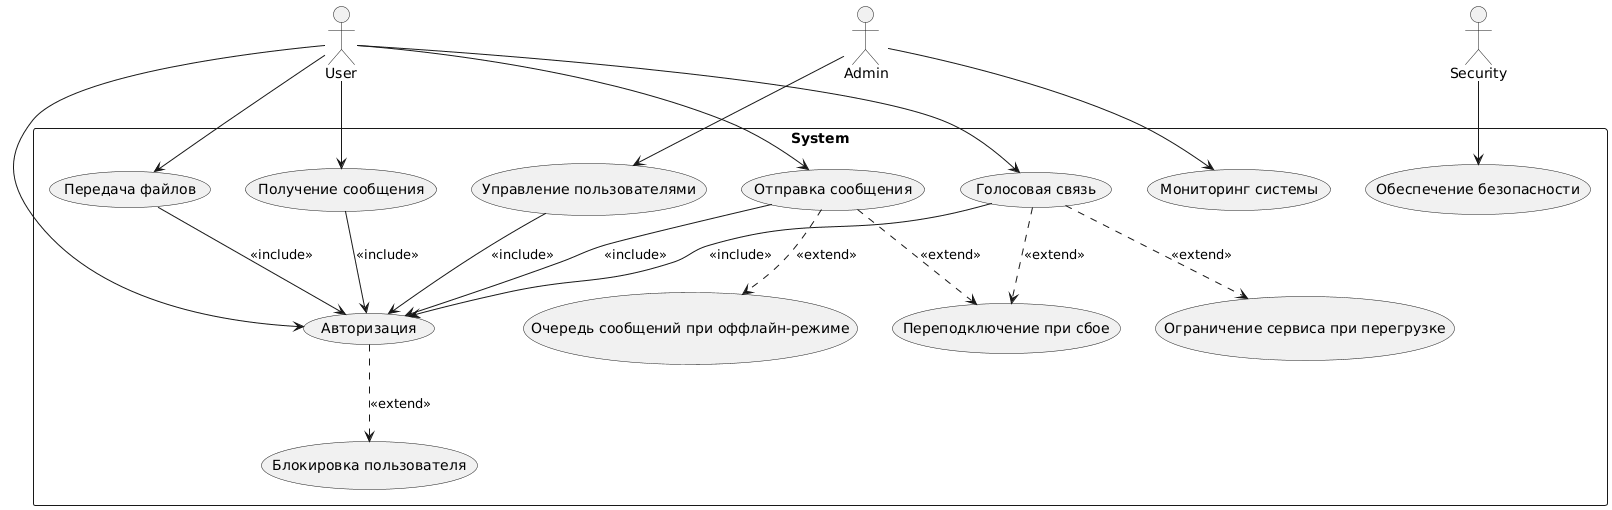
\includegraphics[width=0.78\textwidth]{usecase.png}
    \refstepcounter{figure}
    \caption*{Рисунок \thefigure\ — Диаграмма вариантов использования}
\end{figure}

\section{Описание сценариев вариантов использования}

Для анализа поведения системы корпоративного обмена сообщениями были выбраны
два ключевых варианта использования: авторизация пользователя и отправка
текстового сообщения. Для каждого варианта рассмотрены основные, альтернативные
и исключительные сценарии взаимодействия.

\subsection{Вариант использования «Авторизация пользователя»}

Данный вариант использования описывает процесс аутентификации пользователя в
системе с целью получения доступа к функциональным возможностям корпоративного
мессенджера.

\subsubsection{Основной сценарий}

Основной сценарий предполагает корректное выполнение процедуры входа в систему.

\begin{enumerate}
    \item Пользователь запускает клиентское приложение.
    \item Система отображает форму авторизации.
    \item Пользователь вводит логин и пароль.
    \item Клиентское приложение передаёт данные серверу аутентификации.
    \item Сервер проверяет корректность учётных данных.
    \item Система создаёт пользовательскую сессию и выдаёт токен доступа.
    \item Пользователь получает доступ к интерфейсу обмена сообщениями.
\end{enumerate}

\subsubsection{Альтернативный сценарий}

Альтернативный сценарий возникает при использовании механизма повторной аутентификации.

\begin{enumerate}
    \item Пользователь запускает приложение.
    \item Система обнаруживает действующий токен авторизации.
    \item Выполняется автоматическая проверка срока действия токена.
    \item При успешной проверке пользователь автоматически получает доступ к системе без повторного ввода учётных данных.
\end{enumerate}

\subsubsection{Исключительный сценарий}

Исключительный сценарий связан с ошибкой аутентификации.

\begin{enumerate}
    \item Пользователь вводит логин и пароль.
    \item Сервер выполняет проверку данных.
    \item Обнаруживается несоответствие учётных данных.
    \item Система отклоняет запрос на вход.
    \item Пользователю отображается сообщение об ошибке авторизации.
    \item Пользователь получает возможность повторного ввода данных.
\end{enumerate}

\subsection{Вариант использования «Отправка текстового сообщения»}

Данный вариант использования описывает процесс обмена текстовыми сообщениями между пользователями корпоративной системы.

\subsubsection{Основной сценарий}

Основной сценарий предполагает успешную доставку сообщения.

\begin{enumerate}
    \item Пользователь выбирает чат или адресата.
    \item Пользователь вводит текст сообщения.
    \item Пользователь инициирует отправку сообщения.
    \item Клиентское приложение передаёт сообщение серверу.
    \item Сервер выполняет обработку и маршрутизацию сообщения.
    \item Сообщение сохраняется в системе хранения.
    \item Адресат получает сообщение.
    \item Сообщение отображается в пользовательском интерфейсе обоих участников диалога.
\end{enumerate}

\subsubsection{Альтернативный сценарий}

Альтернативный сценарий возникает при временной недоступности адресата.

\begin{enumerate}
    \item Пользователь отправляет сообщение.
    \item Сервер фиксирует отсутствие активного соединения с адресатом.
    \item Сообщение помещается в очередь доставки.
    \item После восстановления соединения сообщение автоматически доставляется получателю.
\end{enumerate}

\subsubsection{Исключительный сценарий}

Исключительный сценарий связан с потерей соединения с сервером.

\begin{enumerate}
    \item Пользователь инициирует отправку сообщения.
    \item Во время передачи происходит потеря сетевого соединения.
    \item Система фиксирует невозможность доставки.
    \item Сообщение временно сохраняется в локальном буфере клиента.
    \item Пользователю отображается уведомление о проблеме соединения.
    \item После восстановления сети выполняется повторная попытка отправки сообщения.
\end{enumerate}

\section{Диаграммы деятельности}

Диаграмма деятельности авторизации пользователя представлена на рисунке 2.

\begin{figure}[H]
    \label{fig:2}
    \centering
    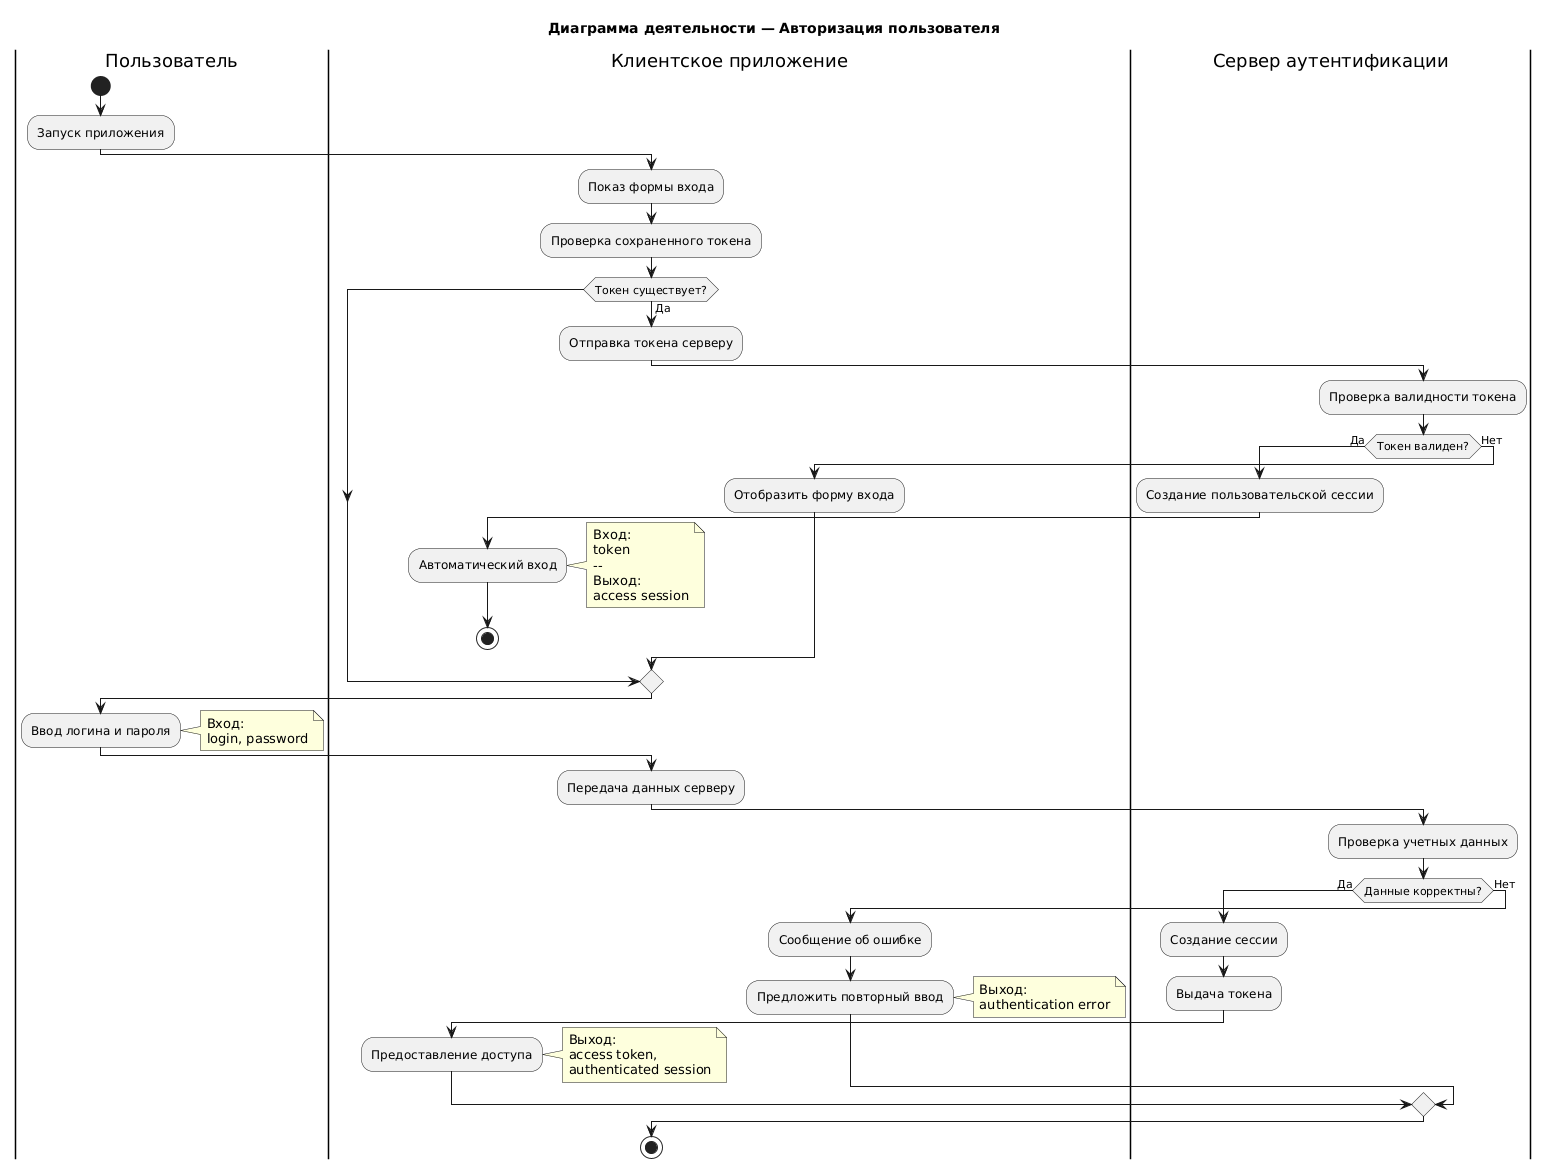
\includegraphics[width=0.78\textwidth]{1.png}
    \refstepcounter{figure}
    \caption*{Рисунок \thefigure\ — Диаграмма деятельности авторизации}
\end{figure}


Диаграмма деятельности отправки сообщения представлена на рисунке 3.

\begin{figure}[H]
    \label{fig:3}
    \centering
    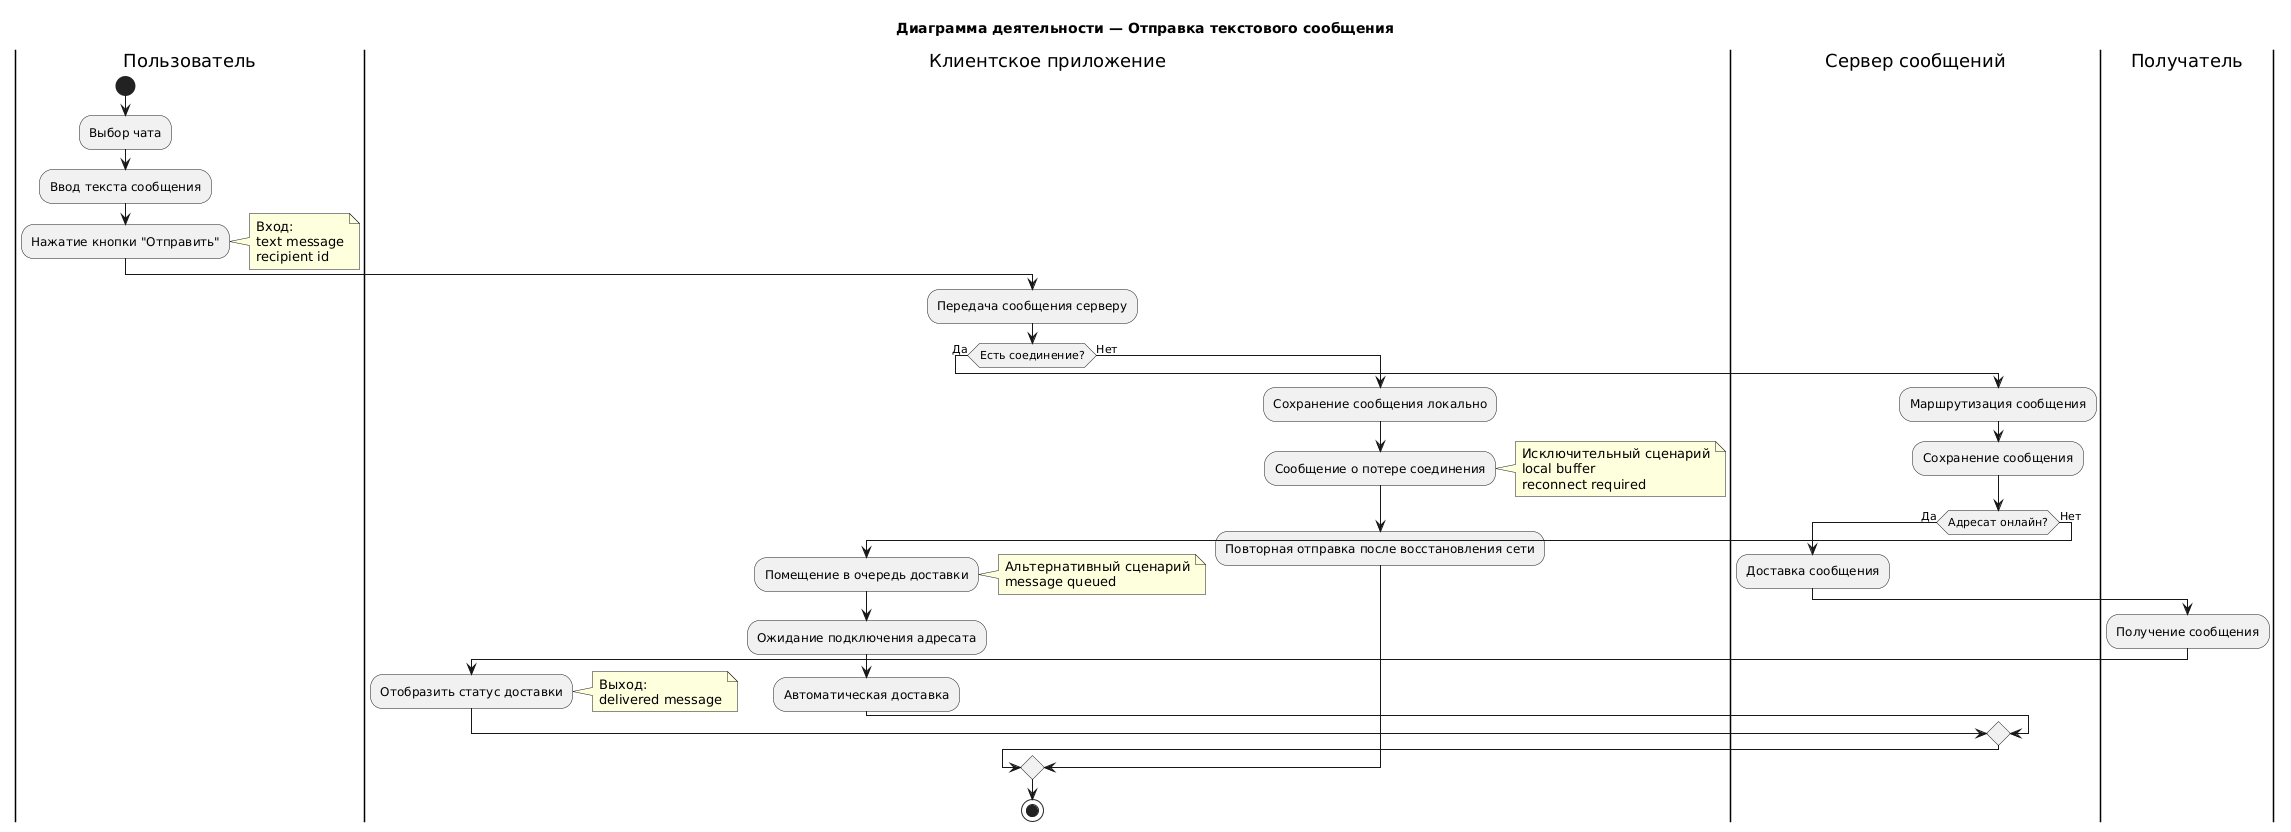
\includegraphics[width=0.78\textwidth]{2.png}
    \refstepcounter{figure}
    \caption*{Рисунок \thefigure\ — Диаграмма деятельности отправки сообщения}
\end{figure}

\end{document}
